%\nonstopmode
\documentclass[12pt]{article}
%\documentclass{article}
\usepackage[utf8]{inputenc}
\usepackage{booktabs}% http://ctan.org/pkg/booktabs
\usepackage{multirow}
\usepackage{microtype}      % microtypography
\usepackage[a4paper, margin=0.78in]{geometry}
\newcommand{\argmax}{\operatornamewithlimits{\mathbb{argmax}}}
\usepackage{amssymb}
\usepackage{breqn}
\usepackage{bm}
\usepackage{wrapfig}
\usepackage{amsmath,eqnarray}
\usepackage[svgnames]{xcolor}
\definecolor{citecol}{RGB}{0,12,128}
\usepackage{bm}
\usepackage{graphicx}
\usepackage[subrefformat=parens,labelformat=parens]{subfig}
\usepackage{float}
\usepackage{mathptmx}
\usepackage[ruled,vlined,linesnumbered]{algorithm2e}
%\usepackage[backend=bibtex,style=alphabetic,citestyle=authoryear]{biblatex}
\usepackage[numbers]{natbib}
\bibliographystyle{abbrv}
% \usepackage{amsmath}
\usepackage{amsfonts}
% \usepackage{hyperref}
\usepackage{yhmath}
\usepackage{colortbl}
\newcommand{\tabitem}{~~\llap{\textbullet}~~}

\newcommand{\xhdr}[1]{{\noindent\bfseries #1}.}
\newcommand{\xit}[1]{{\noindent\textbf{\textit{#1}}}}


\newcommand{\matr}[1]{\mathbf{#1}}
\newcommand{\vect}[1]{\mathbf{#1}}

\newcommand{\va}[0]{\vect{a}}
\newcommand{\vb}[0]{\vect{b}}
\newcommand{\vc}[0]{\vect{c}}
\newcommand{\vd}[0]{\vect{d}}
\newcommand{\ve}[0]{\vect{e}}
\newcommand{\vf}[0]{\vect{f}}
\newcommand{\vg}[0]{\vect{g}}
\newcommand{\vh}[0]{\vect{h}}
\newcommand{\vi}[0]{\vect{i}}
\newcommand{\vm}[0]{\vect{m}}
\newcommand{\vo}[0]{\vect{o}}
\newcommand{\vp}[0]{\vect{p}}
\newcommand{\vq}[0]{\vect{q}}
\newcommand{\vr}[0]{\vect{r}}
\newcommand{\vs}[0]{\vect{s}}
\newcommand{\vv}[0]{\vect{v}}
\newcommand{\vw}[0]{\vect{w}}
\newcommand{\vx}[0]{\vect{x}}
\newcommand{\vy}[0]{\vect{y}}
\newcommand{\vz}[0]{\vect{z}}


\newcommand{\mF}[0]{\matr{F}}
\newcommand{\mH}[0]{\matr{H}}
\newcommand{\mM}[0]{\matr{M}}
\newcommand{\mQ}[0]{\matr{Q}}
\newcommand{\mR}[0]{\matr{R}}
\newcommand{\mU}[0]{\matr{U}}
\newcommand{\mV}[0]{\matr{V}}
\newcommand{\mW}[0]{\matr{W}}

\def\Snospace~{\S{}} % If i don't add this overleaf complains
\renewcommand{\sectionautorefname}{\Snospace}
\renewcommand{\subsectionautorefname}{\Snospace}

% Typography: Define our models here
% Original model
\newcommand{\OR}{$\mathcal{M}_{\texttt{N}}$}
% Random n=1
\newcommand{\RI}{$\mathcal{M}_{\texttt{1}}$}
% Random n=2
\newcommand{\RII}{$\mathcal{M}_{\texttt{2}}$}
% Random n=3
\newcommand{\RIII}{$\mathcal{M}_{\texttt{3}}$}
% Random n=4
\newcommand{\RIV}{$\mathcal{M}_{\texttt{4}}$}
% Random Corpus
\newcommand{\RC}{$\mathcal{M}_{\texttt{UG}}$}
% Random Uniform
\newcommand{\RU}{$\mathcal{M}_{\texttt{UF}}$}
% Random initialization
\newcommand{\RT}{$\mathcal{M}_{\texttt{RI}}$}
% No positional embedding
\newcommand{\NP}{$\mathcal{M}_{\texttt{NP}}$}
% 512 word randomization
\newcommand{\RV}{$\mathcal{M}_{\texttt{512}}$}



%\hypersetup{colorlinks=true,citecolor=citecol}
%\DeclareMathOperator*{\argmax}{arg\,max}

%\addbibresource{syllabus.bib}

\title{Systematic language understanding: a study on the capabilities and limits of language understanding by modern neural networks}
\author{Koustuv Sinha \\ Ph.D. Proposal Document}
\date{September 2021}

\begin{document}

\maketitle

\section{Introduction}

Language allows us to express and comprehend a vast variety of novel thoughts and ideas. Through language, humans exhibit higher-order reasoning and comprehension. Thus, to develop models which mimic human-like reasoning, a principled focus in computer science research is to develop models which understand and reason on natural language. To foster research in developing such state-of-the-art natural language understanding (NLU) models, several datasets and tasks on reading comprehension have been proposed in recent literature. These include tasks such as question answering (QA), natural language inference (NLI), commonsense reasoning to name a few. Over the last decade, several advancements have been made to develop such models, the most successful ones till date involve deep neural models, especially Transformers \CITE, a class of multi-head self-attention models. Since its introduction in 2017, Transformer-based models have achieved impressive results on numerous benchmarks and datasets, with BERT \CITE being one of the most popular instantiation of the same. Using a technique known as ``pre-training'', Transformer-based models are first trained to replicate massive corpus of text. Through this kind of unsupervised training, the models learn and tune their millions and billions of parameters, and using which they solve NLU datasets with surprising, near-human efficiency \CITE.

While Transformer-based models excel in these datasets, it is less clear why do they work so well. Due to the sheer amount of overparameterization, direct inspection of the inner workings of these models are limited. Thus, various research have been conducted by using auxilliary tasks and probing functions to understand the reasoning processes employed by these models \cite{rogers2020}. It has been claimed in the literature that BERT embeddings contain syntactic information about a given sentence, to the extent that the model may internally perform several natural language processing pipeline steps, involving parts-of-speech tagging, entity recognition etc \CITE. BERT has also been credited to acquire some level of semantic understanding \CITE, and contains relevant information about relations and world knowledge \CITE. All of these results indicate to the fact that purely pre-training with massive overparameterized models and large corpora might just be the perfect roadmap to achieve ``human-like'' reasoning capabilities.

On the other hand, there have been growing concerns regarding the ability of these NLU models to understand language in a ``systematic'' and robust way. The phenomenon of \textit{systematicity}, widely studied in the cognitive sciences, refers to the fact that lexical units such as words make consistent contributions to the meaning of the sentences in which they appear \CITE[Fodor]. As an illustration, they provide an example that all English speakers who understand the sentence ``John loves the girl'' should also understand the phrase ``the girl loves John''. In case of NLU tasks, this accounts to model being consistent in understanding novel compositions of existing, learned words or phrases. However, there is growing evidence in literature which highlight the brittleness of NLU systems to such adversarial examples \CITE. More so, there is strong evidence that state-of-the-art NLU models tend to exploit statistical artifacts in datasets, rather than exhibiting true reasoning and generalization capabilities \CITE.

In view of the positive and negative evidences towards Transformers acquiring ``human-like'' natural language understanding capacity, it is very important that we take a step back and carefully examine the reasoning processes of the NLU models in the view of systematicity and robustness. Since these NLU models are now being deployed in production and decision making systems, it is even more prudent to test the models towards systematic understanding in order to avoid catastrophic scenarios. In this proposal, I thus discuss my work till now in my doctoral studies to understand the limits of systematic and robust natural language understanding of NLU models. Concretely, first I discuss our proposed systematicity tests on artificial and natural languages by using first-order logic (FOL), and what we learned from the model using such tests. This involves the following paper:

\begin{itemize}
  \item \textit{CLUTRR: A Diagnostic Benchmark for Inductive Reasoning from Text}, published at Empirical Methods of Natural Language Processing (EMNLP) 2019 (Oral presentation) \cite{sinha2019a}
\end{itemize}

This document briefly discusses about my other related works in this topic, such as in Natural Language Inference, \textit{Probing Linguistic Systematicity} \footnote{Work done as second author.}, published at Association for Computational Linguistics (ACL) 2020 \cite{goodwin2020}; or in proof generation, \textit{Measuring Systematic Generalization in Neural Proof Generation} \cite{gontier2020}, published at Neural Information Processing Systems (NeurIPS) 2020, but not in detail.

Secondly, I discuss our work on understanding the limits of systematicity of NLU models by subjecting these models to scrambled word order sentences, involving the following two papers:

\begin{itemize}
  \item \textit{UnNatural Language Inference}, published at Association for Computational Linguistics (ACL) 2021 (Oral presentation, Outstanding paper award) \cite{sinha2021}
  \item \textit{Masked Language Modeling and the Distributional Hypothesis: Order Word Matters Pre-training for Little}, published at Empirical Methods of Natural Language Processing (EMNLP) 2021 \cite{sinha2021a}
\end{itemize}

This document does not discuss concurrent works on analyzing faithfulness and robustness in translations \cite{parthasarathi2021a} (published at EMNLP 2021), proposed dataset on systematic reasoning on graph neural networks \cite{sinha2020c}, or an unreferenced automatic dialog evaluation framework \cite{sinha2020d} (published at ACL 2020) conducted during my doctoral studies.

% TODO mostly copy/rephrase stuff from my previous papers. Start with a general introduction

% TODO define systematicity

% TODO state why we need to investigate systematicity of NLU models - cite the problem papers

% Related work

% Connect systematicity to generalization

\section{Background: Natural language understanding through Neural approaches}

Natural language is highly ambiguous (syntactic ambiguity, word sense ambiguity, semantic ambiguity) as well as contextual (multiple interpretations based on usage). To understand natural language, neural network based approaches operate on the notion of \textit{distributional semantics} \cite{bordes2013translating}, which captures the meaning of words through vector representation to compose a meaning representation of the sentence or relations. This makes neural network approaches more robust to noise and ambiguity of natural language \cite{bengio2013representation}.

\xhdr{Models} Natural Language Understanding (NLU) models have thus built on top of neural models having distributional vector representation of the lexical items. Further improvements were made to handle the polysemous and context-dependent nature of words by using contextual embeddings through leveraging the sequences of sentences, typically using Recurrent (LSTM, GRU) or Convolutional models (CNN). Models based on Long Short Term Memory (LSTM) became the de-facto standard in NLU, as they can effectively capture the contextual information with locality bias present in natural language. However, its performance is often affected by the long-term dependency problem in several NLU tasks.

Recently, the field of NLP has witnessed a paradigm shift in research with the advent of Transformers \cite{vaswani-etal-2017-attention}. Being a fully-connected multi-head self-attention model, Transformers can directly model the dependency between any two words in a sequence, thus proving to be more powerful and suitable to model long range dependencies of natural language. However, Transformers come with massively increased model parameters, thus requiring significantly large corpus to train and resulting in overfitting on small and medium sized datasets \cite{radford2018improving}.

\xhdr{On the rise of pre-training} With increasing number of model parameters, the requirement to train on large datasets became inevitable - as otherwise it is not possible to fully train the model parameters. However, it is challenging to collect/design NLU tasks of such scale due to extremely expensive annotation costs. In contrast, it is relatively easy to obtain large-scale unlabeled corpora, typically through scraping the internet or collecting all literary works. Thus came the idea of \textit{pre-training}, where this huge, unlabeled data is first leveraged to learn a good representation, and then the resulting model used for NLU tasks. The large, unlabeled data can be leveraged to learn useful word embeddings either using pairwise ranking \cite{collobert}, or through the use of shallow architectures \cite{mikolov}, or by computing global word-word co-occurence statistics \cite{glove}. However, these pre-trained word embeddings are still context-independent, and requires learning context-dependent parameters from scratch on an NLU task. Thus, efforts have been made to pre-train the entire model parameters instead of generating word embeddings by training in a Language Modeling objective (predicting the probability of a word to appear after a sequence of words), using bidirectional LSTM based architectures \cite{peters}. These models are then used to fine-tune on downstream NLU tasks such as text classification \cite{ULMfit}.

More recently, Transformer-based architectures became widely popular with the introduction of BERT \cite{devlin}. BERT is fundamentally a stack of Transformer layers, having multiple self-attention heads. To learn its massive amount of parameters, BERT is pre-trained on unlabeled corpora using two self-supervised objectives: masked language modeling (MLM, predicting the probability of randomly masked input tokens) and next sentence prediction (predicting if two sentences are adjacent to each other). BERT significantly improved the state-of-the art in many NLU tasks - ranging from text classication, question answering, natural language inference, machine translation, summarization etc \cite{qiu2020}.

\xhdr{Analysis and interpretability of NLU models}
The sheer performance of pre-trained Transformer-based models following BERT created a watershed moment in NLU, as these models outperform previous LSTM-based models by a large extent. Due to this success, interest peaked in the community to investigate the inner workings of this largely black box model \cite{rogers2020}. The investigation is primarily done using the tool of \textit{probing}, which is learning a function on top of pre-trained representations to perform targeted assesment of linguistic information \cite{hupkes2018visualisation}. How well this probe learns a given signal can be seen as a proxy for linguistic knowledge encoded in the representations. Using these probes, it has been shown BERT representations contain adequate syntactic, semantic, and world knowledge \cite{rogers2020}.

\xhdr{Systematicity issues in NLU models} Despite the large performance gain and representations containing the necessary linguistic information to process natural language, state-of-the-art NLU models are often subject to scrutiny due to their unsystematic behaviors on specifically crafted test suites. NLU models are repeatedly shown to be brittle when subject to adversarial attacks \cite{jia2016}. NLU models also tend to exploit the statistical irregularities and annotation artefacts \cite{gururangan2018a} of a given datasets, resulting in failure cases on carefully crafted examples \cite{mccoy2019}. My work during my doctoral thesis has been to uncover why these models reason unsystematically using targeted semantic and syntactic tests.



% Language Models

%\subsection{Natural Language Understanding Models}

% Brief oneliners only
% Refer readers to more involved things


%Transformers
% LSTM-based LM

% The rise of pre-training

%\subsection{On the rise of pre-training}

% is this background? looks more like related work
%\subsection{Syntax and Semantics represented in distributed representations}


\section{Contribution 1: Investigating systematicity of NLU models using first order logic}
\label{sec:cont1}

\subsection{Motivation}

An important challenge in NLU is to develop benchmarks which can precisely test a model's capability for robust and systematic generalization. Ideally, we want language understanding systems that can not only answer questions and draw inferences from text, but that can also do so in a systematic, logical and robust way. While such reasoning capabilities are certainly required for many existing NLU tasks, most datasets combine several challenges of language understanding into one, such as co-reference/entity resolution, incorporating world knowledge, and semantic parsing - making it difficult to isolate and diagnose a model's capabilities for systematic generalization and robustness.

\begin{wrapfigure}{r}{0.5\textwidth}
\begin{center}
  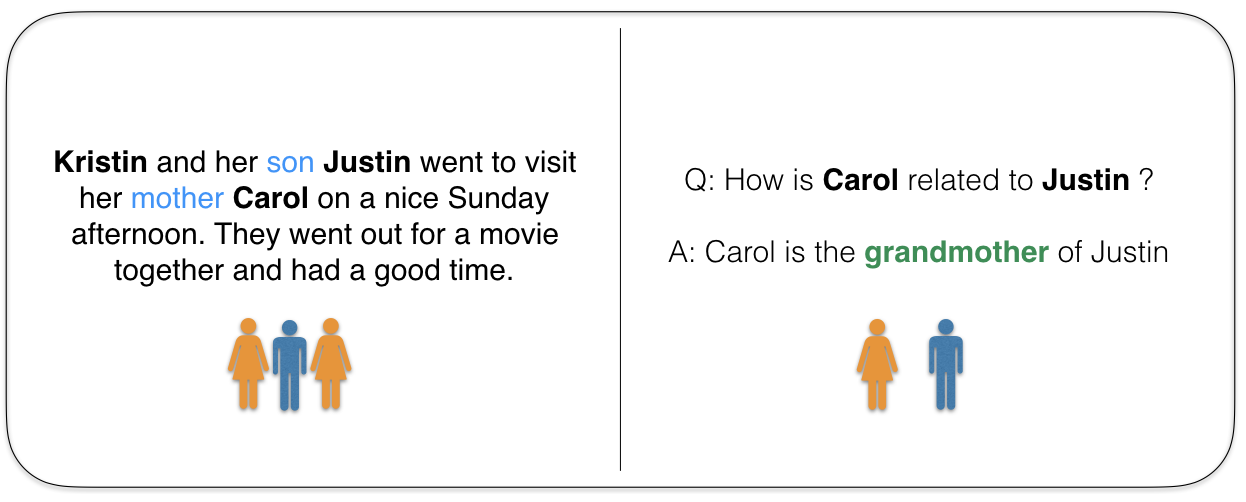
\includegraphics[width=0.48\textwidth]{images/clutrr_text.png}
\end{center}
\caption{CLUTRR inductive reasoning task}
\label{fig:clutrr_data}
\end{wrapfigure}



Thus, inspired by the classic AI challenge of inductive logic programming, we propose a semi-synthetic benchmark designed to explicitly test an NLU model's ability for systematic and robust logical generalization. Our benchmark suite - termed CLUTRR (\textbf{C}ompositional \textbf{L}anguage \textbf{U}nderstanding with \textbf{T}ext-based \textbf{R}elational \textbf{R}easoning) - contains a large set of semi-synthetic stories involving hypothetical families. Given a story, the objective is to infer the relationship between two given characters in the story, whose relationship is not explicitly mentioned. To solve this task, a learning agent must extract the relationships mentioned in the text, induce the logical rules governing the kinship relationships (e.g, the transitivity of the sibling relation), and use rules to infer the relationship between a given pair of entities.

\begin{wrapfigure}{r}{0.5\textwidth}
\begin{center}
  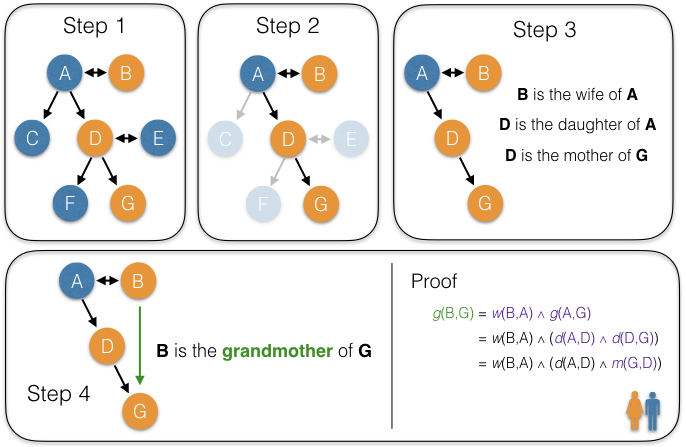
\includegraphics[width=0.48\textwidth]{images/clutrr_dataset_proof.png}
\end{center}
\caption{CLUTRR dataset design steps}
\label{fig:clutrr_data_design}
\end{wrapfigure}

\subsection{Dataset}

In order to design the CLUTRR benchmark, we build upon classic ILP task of inferring kinship relations \cite{hinton1986learning,muggleton1991inductive}. For example, given the facts that \textit{``Alice is Bob's mother''} and \textit{``Jim is Alice's father''}, one can infer with reasonable certainty that \textit{``Jim is Bob's grandfather''}. While this example may appear trivial, it is challenging task to design models that can learn from data to \textit{induce} the logical rules necessary to make such inferences, and it is even more challenging to design models that can systematically generalize by composing these induced rules. Thus, the core idea behind CLUTRR benchmark suite is the following: given a natural language story describing a set of kinship relations, the goal is to infer the relationship between two entities, whose relationship is \textit{not} explicitly stated in the story.

Essentially, we use first order logic (FOL) to generate $k$ number of provable facts and then apply natural language layer on top of it to create a semi-synthetic benchmark. The number $k$ denotes the difficulty of the example. We use Amazon Mechanical Turk (AMT) crowd workers to annotate logical facts into narratives.

% \begin{wrapfigure}{r}{0.5\textwidth}
% \begin{center}
%   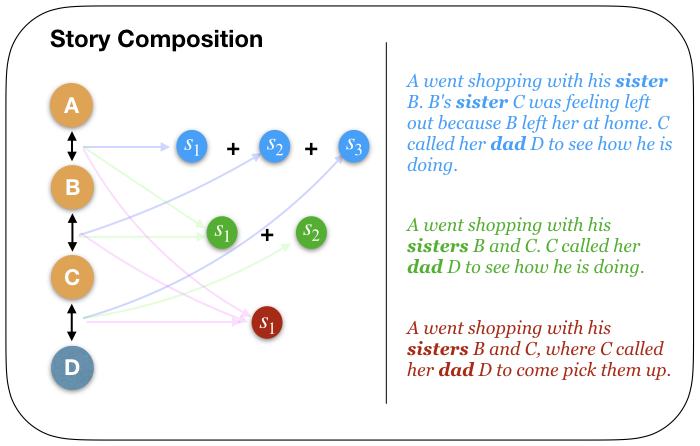
\includegraphics[width=0.48\textwidth]{images/clutrr_composition.png}
% \end{center}
% \caption{Generation of stories by composition in CLUTRR}
% \label{fig:clutrr_composition}
% \end{wrapfigure}

% An example of a story generated by stitching together two shorter paraphrases is provided below:

% \begin{quote}{\small
%     [Frank] went to the park with his father, [Brett]. [Frank] called his brother [Boyd] on the phone. He wanted to go out for some beers.
%     [Boyd] went to the baseball game with his son [Jim].\\
%     Q: What is [Brett] and [Jim]'s relationship?}
% \end{quote}

% Thus, instead of simply collecting paraphrases for a fixed number of stories, we instead obtain a diverse collection of natural language templates that can be programmatically recombined to generate stories with various properties. Please refer to our paper \cite{sinha2019a} for more details about the data generation process.


\subsection{Experiments}

In this section, we use CLUTRR to construct specific instances of the dataset to test various aspects of systematicity in natural language understanding.
We report training and testing results on stories with different clause lengths $k$.
(For brevity, we use the phrase ``clause length'' throughout this section to refer to the number of steps of reasoning that are required to predict the target query.)
We also ensure the AMT templates are also split into train and test, to reduce the probability of overfitting to certain artifacts of the templates.

\xhdr{Human Performance} To get a sense of the data quality and difficulty involved in CLUTRR, we asked human annotators to solve the task for random examples of length $k=2,3,...,6$.
We found that time-constrained AMT annotators performed well (i.e., ${>70\%}$) accuracy for ${k\leq 3}$ but struggled with examples involving longer stories, achieving 40-50\% accuracy for ${k > 3}$. However, trained annotators with unlimited time were able to solve 100\% of the examples (Appendix 1.7), highlighting the fact that this task requires attention and involved reasoning, even for humans.

\xit{Are NLU models able to generalize systematically?}

\begin{wrapfigure}{l}{0.5\textwidth}
\begin{center}
  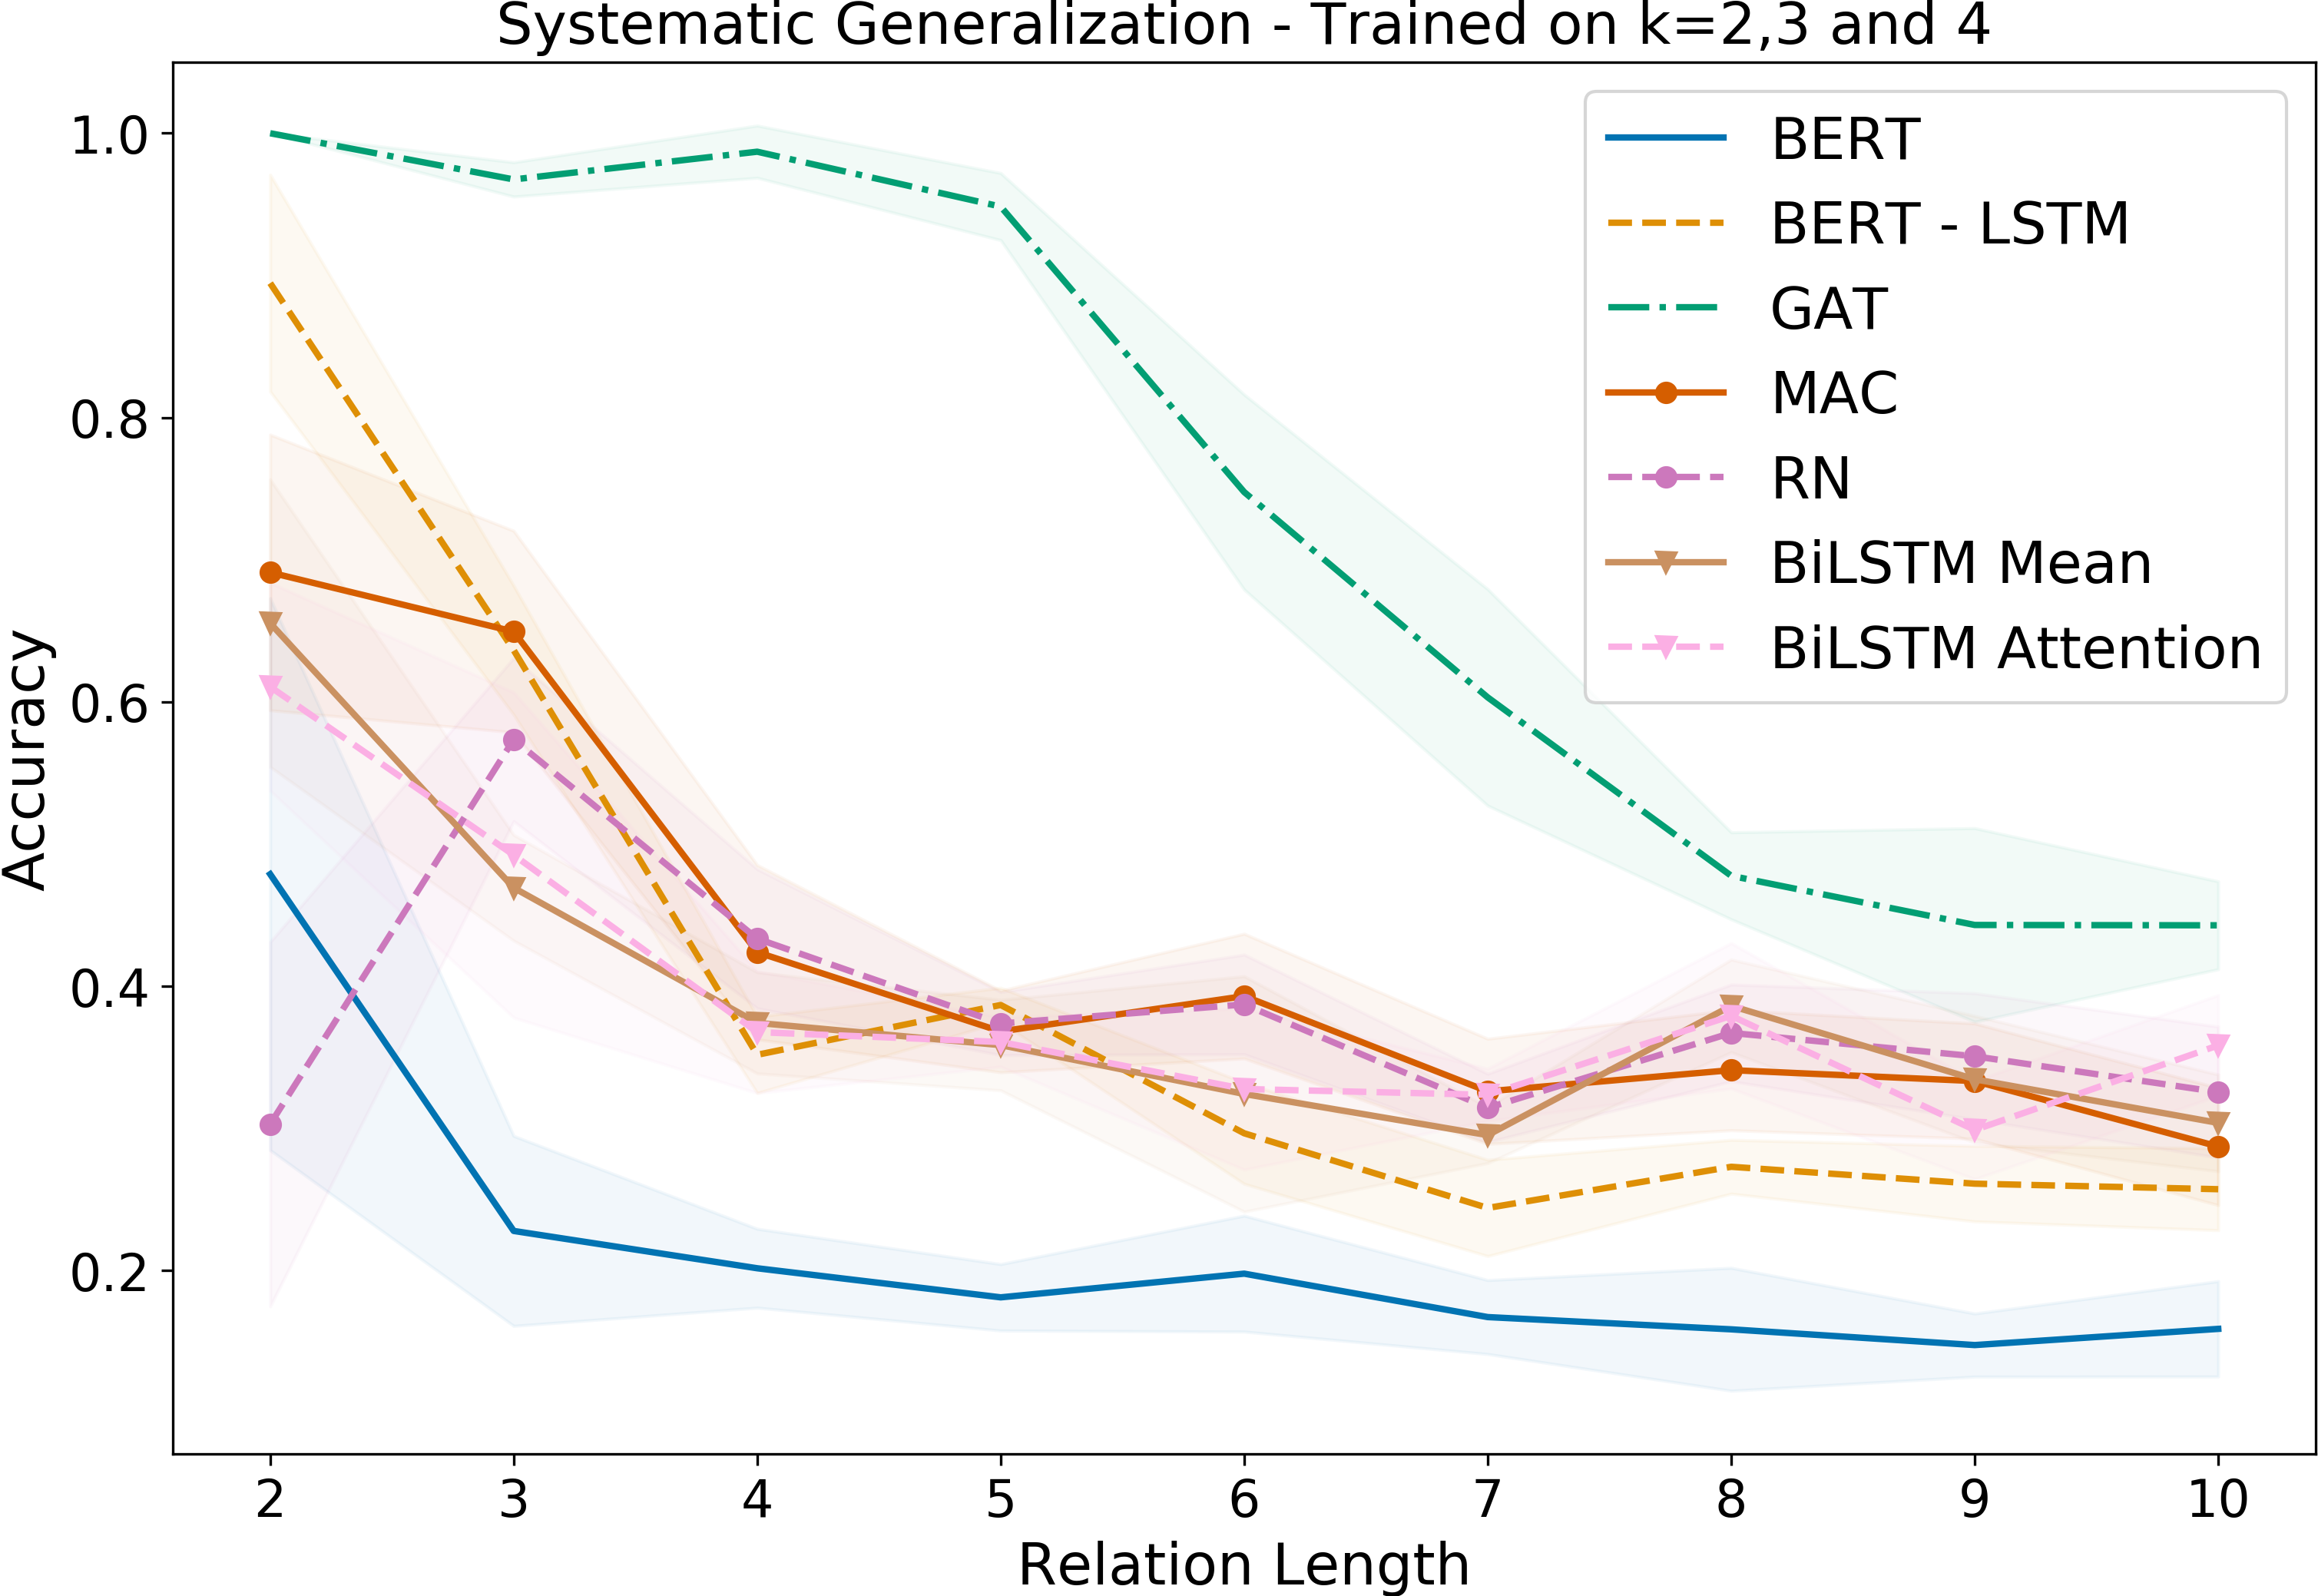
\includegraphics[width=0.48\textwidth]{images/clutrr_sys_gen_234.png}
\end{center}
\caption{Systematic generalization results on CLUTRR, when trained on stories of length $k=2,3,4$}
\label{fig:clutrr_sys_gen_234}
\end{wrapfigure}

In this setup, we consider the setting where the models are trained on stories generated from clauses of length ${\leq k}$ and evaluated on stories generated from larger clauses of length ${>k}$. Thus, we explicitly test the ability for models to generalize on examples that require more steps of reasoning that any example they encountered during training.
In other words, during training, the model sees all logical rules but does not see all {\em combinations} of these logical rules.


Figure \ref{fig:clutrr_sys_gen_234} illustrates the performance of different NLU models on this generalization task. For NLU models, we consider bidirectional LSTMs \citep{hochreiter1997long, cho2014learning} (with and without attention), as well as recently proposed models that aim to incorporate inductive biases towards relational reasoning: Relation Networks (RN) \citep{santoro2017simple} and Compositional Memory Attention Network (MAC) \citep{hudson2018compositional}. We also use the large pretrained language model, BERT \cite{devlin2018bert}, as well as a modified version of BERT having a trainable LSTM encoder on top of the pretrained BERT embeddings. Since the underlying relations in the stories generated by CLUTRR inherently form a graph, we also experiment with a Graph Attention Network (GAT) \citep{Velickovic2017-mh}. Rather than taking the textual stories as input, the GAT baseline receives a structured graph representation of the facts that underlie the story.

We observe that the GAT model is able to perform near-perfectly on the held-out logical clauses of length $k=3$, with the BERT-LSTM being the top-performer among the text-based models but still significantly below the GAT.
Not surprisingly, the performance of all models degrades monotonically as we increase the length of the test clauses, which highlights the challenge of ``zero-shot'' systematic generalization \cite{lake2017generalization, 2018arXiv181107017S}.
GAT, having access to structured input, is able to generalize significantly better compared to NLU models.


% \xhdr{\textit{Is there any benefit to structured input for generalization?}}

% The empirical results on systematic generalization also provide insight into how the text-based NLU systems compare against the graph-based GAT model that has full access to the logical graph structure underlying the stories. Indeed, the relatively strong performance of the GAT model (Figure \ref{fig:gen_1}) suggests that the language-based models fail to learn a robust mapping from the natural language narratives to the underlying logical facts.

% To further confirm this trend, we ran experiments with modified train and test splits for the text-based models, where the same set of natural language paraphrases were used to construct the narratives in both the train and test splits (see our paper \cite{sinha2019a} for details). In this simplified setting, the text-based models must still learn to reason about held-out logical patterns, but the difficulty of parsing the natural language is essentially removed, as the same natural language paraphrases are used during testing and training. We found that the text-based models were competitive with the GAT model in this simplified setting, confirming that the poor performance of the text-based models on the main task is driven by the difficulty of parsing the unseen natural language narratives.


\xit{How does NLU systems cope with noise - how robustly do they reason?}

Finally, we use CLUTRR to systematically evaluate how NLU models cope with noise.
Any set of supporting facts generated by CLUTRR can be interpreted as a path in the corresponding kinship graph $G$ (Figure \ref{fig:clutrr_data_noise}).
Based on this interpretation, we view adding noise facts to the \textit{clean path} from the perspective of sampling three different types of noise paths, from the kinship graph $G$. First, we test for \textit{irrelevant facts}, which consists of facts which has one entity common with the path, but they themselves are irrelevant to solve the task. Second, we test for \textit{supporting facts}, which contain a set of facts which can be used to construct an alternate path between the source and sink (i.e, target entities). Finally, we test for \textit{disconnected facts}, which contain facts which are irrelevant as well as do not contain any entities which are in the path.

\begin{wrapfigure}{l}{0.5\textwidth}
\begin{center}
  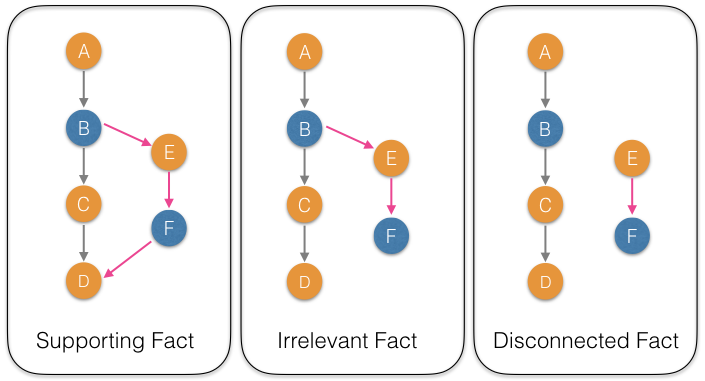
\includegraphics[width=0.48\textwidth]{images/clutrr_noise.png}
\end{center}
\caption{Noise generation methods in CLUTRR}
\label{fig:clutrr_data_noise}
\end{wrapfigure}


\begin{table}[t!]
\caption{Testing the robustness of the various models when training and testing on stories containing various types of noise facts.}
\label{tab:robust}
\resizebox{\textwidth}{!}{
% Please add the following required packages to your document preamble:
% \usepackage{multirow}
\begin{tabular}{@{}cccccccc|c@{}}
\toprule
\multicolumn{1}{l}{} & \multicolumn{1}{l}{Models} & \multicolumn{6}{c}{Unstructured models (no graph)} & \multicolumn{1}{l}{Structured model (with graph)} \\ \midrule
\multicolumn{1}{l}{Training} & \multicolumn{1}{l|}{Testing} & BiLSTM - Attention & BiLSTM - Mean & RN & MAC & \multicolumn{1}{l}{BERT} & \multicolumn{1}{l|}{BERT-LSTM} & GAT \\ \midrule
Clean & \multicolumn{1}{c|}{Clean} & 0.58 \tiny $\pm 0.05$ & 0.53 \tiny $\pm 0.05$ & 0.49 \tiny $\pm 0.06$ & 0.63 \tiny $\pm 0.08$ & 0.37 \tiny $\pm 0.06$ & 0.67 \tiny $\pm 0.03$ & \textbf{1.0} \tiny $\pm 0.0$ \\
 & \multicolumn{1}{c|}{Supporting} & \textbf{0.76} \tiny $\pm 0.02$ & 0.64 \tiny $\pm 0.22$ & 0.58 \tiny $\pm 0.06$ & 0.71 \tiny $\pm 0.07$ & 0.28 \tiny $\pm 0.1$ & 0.66 \tiny $\pm 0.06$ & 0.24 \tiny $\pm 0.2$ \\
 & \multicolumn{1}{c|}{Irrelevant} & 0.7 \tiny $\pm 0.15$ & \textbf{0.76} \tiny $\pm 0.02$ & 0.59 \tiny $\pm 0.06$ & 0.69 \tiny $\pm 0.05$ & 0.24 \tiny $\pm 0.08$ & 0.55 \tiny $\pm 0.03$ & 0.51 \tiny $\pm 0.15$ \\
 & \multicolumn{1}{c|}{Disconnected} & 0.49 \tiny $\pm 0.05$ & 0.45 \tiny $\pm 0.05$ & 0.5 \tiny $\pm 0.06$ & 0.59 \tiny $\pm 0.05$ & 0.24 \tiny $\pm 0.08$ & 0.5 \tiny $\pm 0.06$ & \textbf{0.8} \tiny $\pm 0.17$ \\ \midrule
Supporting & \multicolumn{1}{c|}{Supporting} & 0.67 \tiny $\pm 0.06$ & 0.66 \tiny $\pm 0.07$ & 0.68 \tiny $\pm 0.05$ & 0.65 \tiny $\pm 0.04$ & 0.32 \tiny $\pm 0.09$ & 0.57 \tiny $\pm 0.04$ & \textbf{0.98} \tiny $\pm 0.01$ \\
\midrule
Irrelevant & \multicolumn{1}{c|}{Irrelevant} & 0.51 \tiny $\pm 0.06$ & 0.52 \tiny $\pm 0.06$ & 0.5 \tiny $\pm 0.04$ & 0.56 \tiny $\pm 0.04$ & 0.25 \tiny $\pm 0.06$ & 0.53 \tiny $\pm 0.06$ & \textbf{0.93} \tiny $\pm 0.01$ \\
\midrule
Disconnected & \multicolumn{1}{c|}{Disconnected} & 0.57 \tiny $\pm 0.07$ & 0.57 \tiny $\pm 0.06$ & 0.45 \tiny $\pm 0.11$ & 0.4 \tiny $\pm 0.1$ & 0.17 \tiny $\pm 0.05$ & 0.47 \tiny $\pm 0.06$ & \textbf{0.96} \tiny $\pm 0.01$ \\ \midrule
  \multicolumn{1}{l}{Average} & \multicolumn{1}{c|}{} & \textbf{0.61} \tiny $\pm 0.08$ & 0.59 \tiny $\pm 0.08$ & 0.54 \tiny $\pm 0.07$ & \textbf{0.61} \tiny $\pm 0.06$ & 0.30 \tiny $\pm 0.07$ & 0.56 \tiny $\pm 0.05$ & \textbf{0.77} \tiny $\pm 0.09$ \\ \bottomrule
\end{tabular}}
\end{table}


Overall, we find that the GAT baseline outperforms the unstructured text-based models across most testing scenarios (Table \ref{tab:robust}), which showcases the benefit of a structured feature space for robust reasoning.
When training on clean data and testing on noisy data, we observe two interesting trends that highlight the benefits and shortcomings of the various model classes. Firstly, all the text-based models excluding BERT actually perform better when testing on examples that have {\em supporting} or {\em irrelevant} facts added. This suggests that these models actually benefit from having more content related to the entities in the story. Even though this content is not strictly useful or needed for the reasoning task, it may provide some linguistic cues (e.g., about entity genders) that the models exploit. In contrast, the BERT-based models do not benefit from the inclusion of this extra content, which is perhaps due to the fact that they are already built upon a strong language model (e.g., that already adequately captures entity genders.)
Secondly, the GAT model performs poorly when {\em supporting} facts are added but has no performance drop when {\em disconnected} facts are added. This suggests that the GAT model is sensitive to changes that introduce cycles in the underlying graph structure but is robust to the addition of noise that is disconnected from the target entities.
Moreover, when we trained on noisy examples, we found that only the GAT model was able to consistently improve its performance (Table \ref{tab:robust}).
Again, this highlights the performance gap between the unstructured text-based models and the GAT.

\subsection{Discussion}

In this paper we introduced the CLUTRR benchmark suite to test the systematic generalization and inductive reasoning capababilities of NLU systems.
We demonstrated the diagnostic capabilities of CLUTRR and found that existing NLU systems exhibit relatively poor robustness and systematic generalization capabilities---especially when compared to a graph neural network that works directly with symbolic input.
These results highlight the gap that remains between machine reasoning models that work with unstructured text and models that are given access to more structured input.
We hope that by using this benchmark suite, progress can be made in building more compositional, modular, and robust NLU systems.

\subsection{Related Works}

We also conduct a couple of related studies in testing systematicity of Natural Language Understanding (NLU) and Natural Language Generation (NLG) models following the intuition gained from CLUTRR.

\xhdr{\textit{Probing Linguistic Systematicity}} \cite{goodwin2020} In this work, we introduce several novel probes for testing systematic generalization in Natural Language Inference (NLI). Systematicity is the property whereby words have consistent contributions to composed meaning of the sentences. In this work, we employed an artificial, controlled language where we use \textit{Jabberwocky}-type \footnote{Jabberwocky is the term coined by Lewis Caroll in his poem, which combibes nonsense words with familiar words in a way that allows speakers to recognize the expression as well formed.} sentences to inspect the generalizability of word representations learned by neural networks. We gradually and systematically expose the NLU model to new, \textit{open-class} words in context of NLI tasks, and test whether this exposure alters the systematic understanding of existing, known \textit{closed-class} words. For example, we might train an NLI models with the premise-hypothesis contradiction pair \textit{All pigs sleep; some pigs don't sleep}, and test whether the network can identify the contradiction pair \textit{All Jabberwocks flug; some Jabberwocks don't flug}. A systematic learner would reliably identify the contradiction, whereas a non-systematic learner may allow the closed-class words (\textit{all, some, don't}) to take contextually conditioned meanings that depend on novel context words.

\begin{table*}[h]
  \centering
  \resizebox{\textwidth}{!}{
    \begin{tabular}{|l||llllll|}
      \hline
        \textbf{Position} & 1 & 2 & 3 &  4 & 5 & 6 \\ \hline
  \rowcolor{gray!6} \textbf{Category} & \texttt{quantifier} & \texttt{nominal premodifier} & \texttt{noun} &  \texttt{nominal postmodifier} & \texttt{negation} & \texttt{verb}  \\
  \textbf{Status} & Obligatory & Optional & Obligatory &  Optional & Optional & Obligatory\\
  \rowcolor{gray!6} \textbf{Class} & Closed & Closed & Open & Closed & Closed & Open \\
  \textbf{Example} & {\Large \exam{All}} &  {\Large \exam{brown}} &  {\Large  \exam{dogs}} &  {\Large  \exam{that bark}} &  {\Large \exam{don't}} &  {\Large \exam{run}} \\
  \hline
\end{tabular}
}
\caption{A template for sentences in the artificial language. Each sentence fills the obligatory positions 1, 3, and 6 with a word: a quantifier, noun, and verb. Optional positions (2, 4 and 5) are filled by either a word (adjective, postmodifier or negation) or by the empty string. Closed-class categories (Quantifiers, adjectives, post modifiers and negation) do not include novel words, while  open-class categories (nouns and verbs) includes novel words that are only exposed in the test set.
} \label{tbl:artlang}
\end{table*}


Concretely, we construct an artificial language with six-position template which includes a quantifier (position 1), noun (position 3), and a verb (position 6) with options pre- and post-modifiers (position 2 and 4) and optional negation (position 5). To mimic real world topicality, we contruct \textit{block} structures consisting of nouns and verbs having taxonomic relationships (such as \textit{lizards/animals. run/move}). Nouns and verbs from different blocks have no relationships (such as \textit{lizards} and \textit{screwdrivers} or \textit{run} and \textit{read}). The same set of closed-class words appear in all blocks with consistent meanings. We analyze several state-of-the-art NLI models such as Bidirectional LSTM, InferSent, self-attentive sentence encoder (SATT) and Hierarchical Convolutional Networks (CONV) \footnote{Since the first version of the paper was done prior to the popularity of BERT, we were unable to test the systematicty of BERT-based models in this work. However, our database and code are online, and it would be trivial to use pre-trained BERT models to run the same experiments.}.

We observed all models to perform substantially worse on probing tasks, with standard deviation being significantly high among various blocks - indicating unsystematic behavior. Closed-class words do not maintain a consistent intepretation when paired with different open-class words. Variance across blocks shows that under all models the behaviour of closed-class words is highly sensitive to the novel words they appear with. Thus, our experiments highlight that fact their despite high overall performance, state-of-the-art NLU models generalize in ways that allow the meanings of individual words to vary in different contexts, even in an artificial language where a totally systematic solution is available.

\xhdr{\textit{Measuring Systematic Generalization in Neural Proof Generation with Transformers}} \cite{gontier2020} In this work, we extend our systematicity analysis to language generation using Transformer Language Models (TLMs). To analyze systematicity, we re-use our CLUTRR benchmark to conduct proof generation using forward and backward chaining concepts in first-order logic (FOL). For example, a set of facts in CLUTRR could be of the form: \textit{``Nat is the granddaughter of Betty'', ``Greg is the brother of Nat'', ``Flo is the sister of Greg''}, where the relationship among \textit{Flo} and \textit{Betty} can be inferred using logical deduction (\textit{``Flo is the granddaughter of Betty''}). In this example, we further task the TLM to generate a plausible proof along with the answer : \textit{``Since Flo is the sister of Greg, and Nat is the granddaughter of Betty, and Greg is the brother of Nat, then Flo is the granddaugher to Betty''}.

In our work, we evaluate two popular proof resolution strategies used in Inductive Logic Programming \cite{Evans2017-pu} , \textit{forward} and \textit{backward} chaining resolution paths, expressed in natural language. We evaluate the validity of the proof and the answer accuracy on various settings: whether the TLM is tasked to generated forward or backward proofs, whether the TLM is provided with a gold proof, or when the TLM is neither provided nor tasked to generate a proof. We train a Transformer \cite{vaswani2017attention} model on scratch on the training set, and we observe that TLMs are only able to generalize to unseen proof steps in case of \textit{interpolation}, that is when stories of lesser difficulties than training are provided during inference. In case of \textit{extrapolation}, we observe similar generalization issues as in CLUTRR, where models fail to generalize beyond the difficulty trained. In terms of proof understanding, we observed backward chaining proofs are better understood by the model than forward chaining for the TLMs, mostly due to the fact that backward chaining proofs always begings with the target answer first, allowing the model to exploit the positional cues. Surprisingly, we found the no proof situation to have better answer accuracy than in the case of proof generation - alluding to the fact that proof generation might be actually deterioriating the model performance as it requires more involved reasoning.

\begin{wrapfigure}{l}{0.5\textwidth}
\begin{center}
  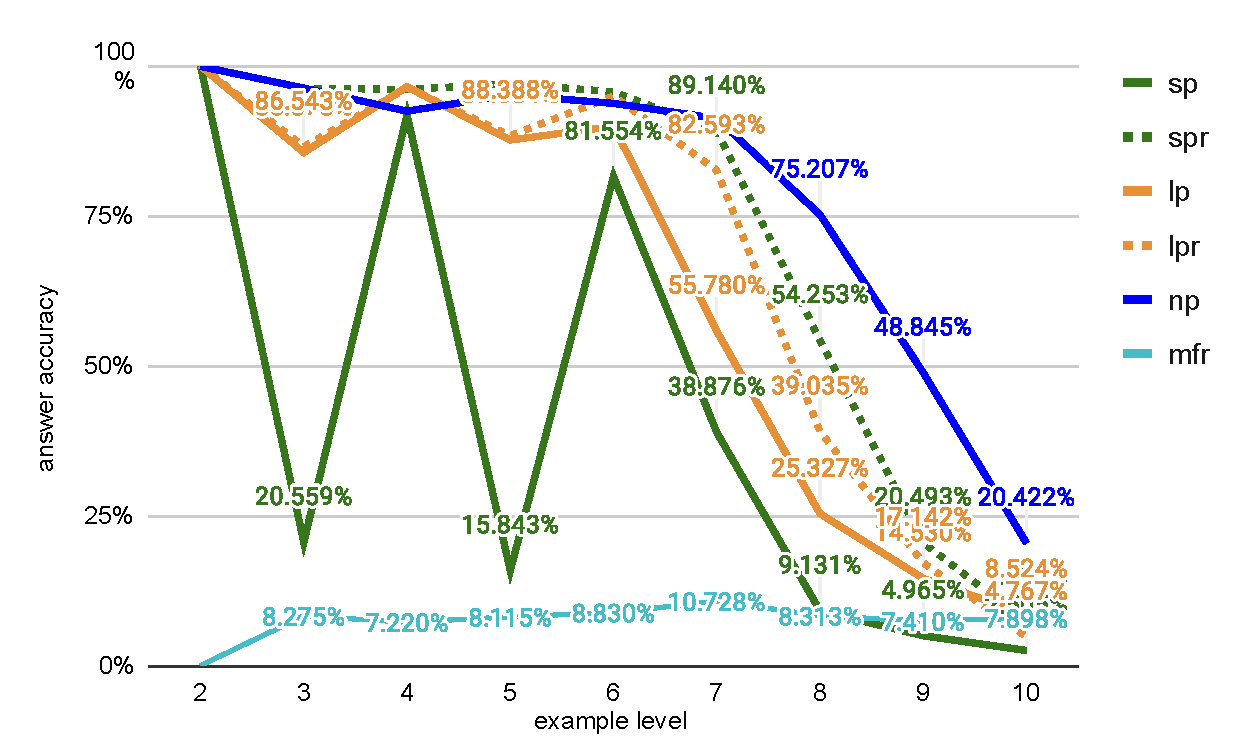
\includegraphics[width=0.48\textwidth]{images/proof_sys_gen.pdf}
\end{center}
\caption{Systematic generalization issues in proof generation}
\label{fig:proof_sys_gen}
\end{wrapfigure}


Finally, in proof generation, we found forward-chaining generation is easier for TLM than backward chaining generation. This is contrary to our previous observation, and we believe this is due to the fact that the model has a higher chance of generating the first proof step correctly than the final proof step. Overall, TLMs are unable to generate valid proofs of unseen lengths, both in \textit{interpolation} and \textit{extrapolation} setting. However, when provided with the correct proof, TLMs are better able to exploit the information in it to be better at systematic generalization. Our results highlight multiple insights - first, TLMs suffer length generalization issues in proof generation, and TLMs get better at reasoning when provided with correct proofs. Our framework can thus be used to easily analyze systematicity issues in generation as it is grounded with first-order logic.

\section{Contribution 2: Probing systematicity of pre-trained models using word order}
\label{sec:cont2}

As we uncover the systematicity issues in state-of-the-art NLU models, one question emerges - does the unsystematic behaviour of NLU models stem from their inability to understand syntax? Since we use artificial and semi-synthetic datasets in all our prior works, having a rudimentary variation of syntax, our  findings naturally raise questions on the actual syntax understanding capabilities of NLU models. Of late, we have witnessed a steady increase in performance of large scale pre-trained Transformer-based \cite{vaswani-etal-2017-attention} models---such as RoBERTa \cite{liu-et-al-2019-roberta}, BART \cite{lewis-etal-2020-bart}, and GPT-2 and -3 \cite{radford-etal-2019-language,brown-etal-2020-gpt3}--on many NLU tasks \cite{wang-etal-2018-glue, wang-etal-2019-superglue}. The success of these models has prompted serious investigation, leading claims that a language modeling (LM) objective can capture syntactic information \cite{hewitt-manning-2019-structural,jawahar-etal-2019-bert, warstadt-bowman-2020-can, wu-etal-2020-perturbed}, with their self-attention layers being capable of surprisingly effective learning \cite{rogers2020}.

In the following section, we discuss two related works \cite{sinha2021,sinha2021a} on testing systematicity of syntax understanding of NLU models using the proxy of \textit{word order}.

\subsection{UnNatural Language Inference}

\subsubsection{Motivation}

In this contribution, \cite{sinha2021} we revisit the notion of ``knowing syntax'' under the lens of systematicity. A natural and common perspective from many formal theories of linguistics (e.g., \cite{chomsky-1995-minimalist}) is that knowing a natural language requires that you know the syntax of that language. Knowing the syntax of a sentence means being sensitive to the \textit{order of the words} in that sentence (among other things).  Humans are sensitive to word order, so clearly, ``language is not merely a bag of words'' \cite[p.156]{harris-1954-distributional}.
Moreover, it is easier for us to identify or recall words presented in canonical orders than in disordered, ungrammatical sentences; this phenomenon is called the \textit{``sentence superiority effect''} (\cite{cattell-1886-time, scheerer1981early, toyota-2001-changes, baddeley-etal-2009-working, snell-grainger-2017-sentence, snell2019word, wen-etal-2019-parallel}, i.a.).
In our estimation then, if one wants to claim that  a model ``knows syntax'', then they should minimally show that the model is sensitive to word order (at least for e.g. English or Mandarin Chinese).

Generally, knowing the syntax of a sentence is taken to be a prerequisite for understanding what that sentence means \cite{heim-kratzer-1998-semantics}.
Models should have to know the syntax first then, if performing any particular NLU task that genuinely requires a humanlike understanding of meaning (cf. \cite{bender-koller-2020-climbing}).
Thus, if our models are as good at NLU as our current evaluation methods suggest, we should expect them to be sensitive to word order (see \autoref{tab:example}).  We find, based on a suite of permutation metrics, that they are not.

\subsubsection{Experiments and Results}

\begin{wraptable}{r}{0.5\textwidth}
    \centering
    \small
    \resizebox{0.5\textwidth}{!}{
    \begin{tabular}{p{11em}p{9em}p{3em}} % I hate the vertical line, can we get rid of it...
    \toprule
     \bf Premise & \bf Hypothesis & \bf Predicted Label \\ \midrule
    Boats in daily use lie within feet of the fashionable bars and restaurants.  & There are boats close to bars and restaurants. & E \\
    \addlinespace[0.5em]
    restaurants and use feet of fashionable lie the in Boats within bars daily . & bars restaurants are There and to close boats . & E \\ \midrule
    He and his associates weren't operating at the level of metaphor. & He and his associates were operating at the level of the metaphor. & C\\  \addlinespace[0.5em]
    his at and metaphor the of were He operating associates n't level . & his the and metaphor level the were He at associates operating of . & C\\
    \bottomrule
    \end{tabular}}
    \caption{Examples from the MNLI Matched development set. Both the original example and the permuted one elicit the same classification label (entailment and contradiction respectively) from RoBERTa (large).}
    \label{tab:example}
\end{wraptable}



We focus here on textual entailment, one of the hallmark tasks used to measure how well models understand language \cite{condoravdi-etal-2003-entailment, dagan-etal-2005-pascal}. This task, often also called Natural Language Inference (NLI; \cite{bowman-etal-2015-large}, i.a.), typically consists of two sentences: a premise and a hypothesis. The objective is to predict whether the premise entails the hypothesis, contradicts it, or is neutral with respect to it.

We find rampant word order insensitivity in purportedly high performing NLI models. For nearly all premise-hypothesis pairs, \textbf{there are many permuted examples that fool the models} into providing the correct prediction. In case of MNLI, for example, the current state-of-the-art of 90.5\% can be increased to \textbf{98.7}\% merely by permuting the word order of test set examples. We even find drastically increased cross-dataset generalization when we reorder words. This is not just a matter of chance---we show that the model output probabilities are significantly different from uniform.
We verify our findings with three popular English NLI datasets---SNLI \citep{bowman-etal-2015-large}, MultiNLI \citep{williams-etal-2018-broad} and ANLI \citep{nie-etal-2020-adversarial})---
and one Chinese one, OCNLI \cite{hu-etal-2020-ocnli}. It is thus less likely that our findings result from some quirk of English or a particular tokenization strategy.
We also observe the effect for various transformer architectures pre-trained on language modeling (BERT, RoBERTa, DistilBERT), and non-transformers, including a ConvNet, an InferSent model, and a BiLSTM.

% \xit{How to construct permuted examples?}

% For any sentence pair in the NLI dataset, we use a permutation function $\mathcal{F}$ which essentially permutes the word order of a sentence with the restriction that no words maintain their original position. Thus, if a sentence $S$ contains $w$ words, then the total number of available permutations of $S$ are $(w-1)!$. This allows us to inspect \textit{multiple} permutations per hypothesis-premise pair. Concretely, we always test using 100 unique permutations for each hypothesis-premise pair in the NLI dataset. If a given NLU model (RoBERTa/BART/DistilBERT/InferSent/ConvNet/BiLSTM) assigns the gold label to \textit{any one} permutation of an hypothesis-premise pair, we mark that example as correct to compute Maximum Accuracy, $\Omega_{\text{max}}$. Now, this metric is strict as it does not allow for any permutation to be processed by the NLU model. We further relax this metric to $\Omega_{\text{rand}}$, where a hypothesis-premise is marked correct if more than 1/3rd of its permutations are assigned the gold label by the model. Going down this route, we can define metrics until $\Omega_{1.0}$, where \textit{all} permutations of an example are assigned the gold label. A graphical representation of the metrics are provided in Figure. Additionally, we also compute the probability of acceptance given a base condition: how many permutations are assigned gold label when the example satisfies this base condition. We use the original model accuracy as the base condition - allowing us to compute $P^{c}$ (probability of correctness)/$P^{f}$ (probability of flips) - given the example is originally predicted correctly/incorrectly by the model, what is the probability of its permutations to be assigned the gold label.

\xit{How many permuted examples does the model accept?}

We find for models trained and evaluated on MNLI (in-domain generalization), there exists at least one permutation for each example using which we can reach a \textit{maximum accuracy} of \textbf{98.7\%} on MNLI dev. and test sets (in RoBERTa, compared to \textit{original accuracy} of 90.6\% in the natural data. If we choose examples such that at least 33\% of its permutations are assigned the gold label (random baseline), we can still cover 79.4\% of the test set (\textit{random accuracy}, see our paper \cite{sinha2021a} for more details on the construction of the metrics.)
We observe the effect even in out-of-domain generalization with ANLI dataset, where the data splits resulted in a maximum accuracy value that is notably higher than the original accuracy (89.7\% vs 45.6\% for RoBERTa). As a consequence, we encounter many \textit{flips}, i.e., examples where the model is unable to predict the gold label, but at least one permutation of that example is able to. However, recall this analysis expects us to know the gold label upfront, so this test can be thought of as running a word-order probe test on the model until the model predicts the gold label (or give up by exhausting our set of 100 permutations). For out-of-domain generalization, random accuracy decreases considerably (36.4\% on A1). Overall, we find the \textit{probability of acceptance} of permutations to be significantly high, suggesting a bag-of-words (BoW) likeness of the models. We find this BOW-likeness to be higher for certain non-Transformer models, (InferSent) (84.2\% for InferSent compared to 70.7\% for RoBERTa on MNLI). We extended the experiments to the Original Chinese NLI dataset \citep[OCNLI]{hu-etal-2020-ocnli}, and re-used the pre-trained RoBERTa-Large and InferSent (non-Transformer) models on OCNLI. Our findings are similar to the English results, thereby suggesting that the phenomenon is not just an artifact of English text or tokenization.


\xit{How confident are models in accepting permuted examples?}

\begin{wrapfigure}{r}{0.5\textwidth}
\begin{center}
  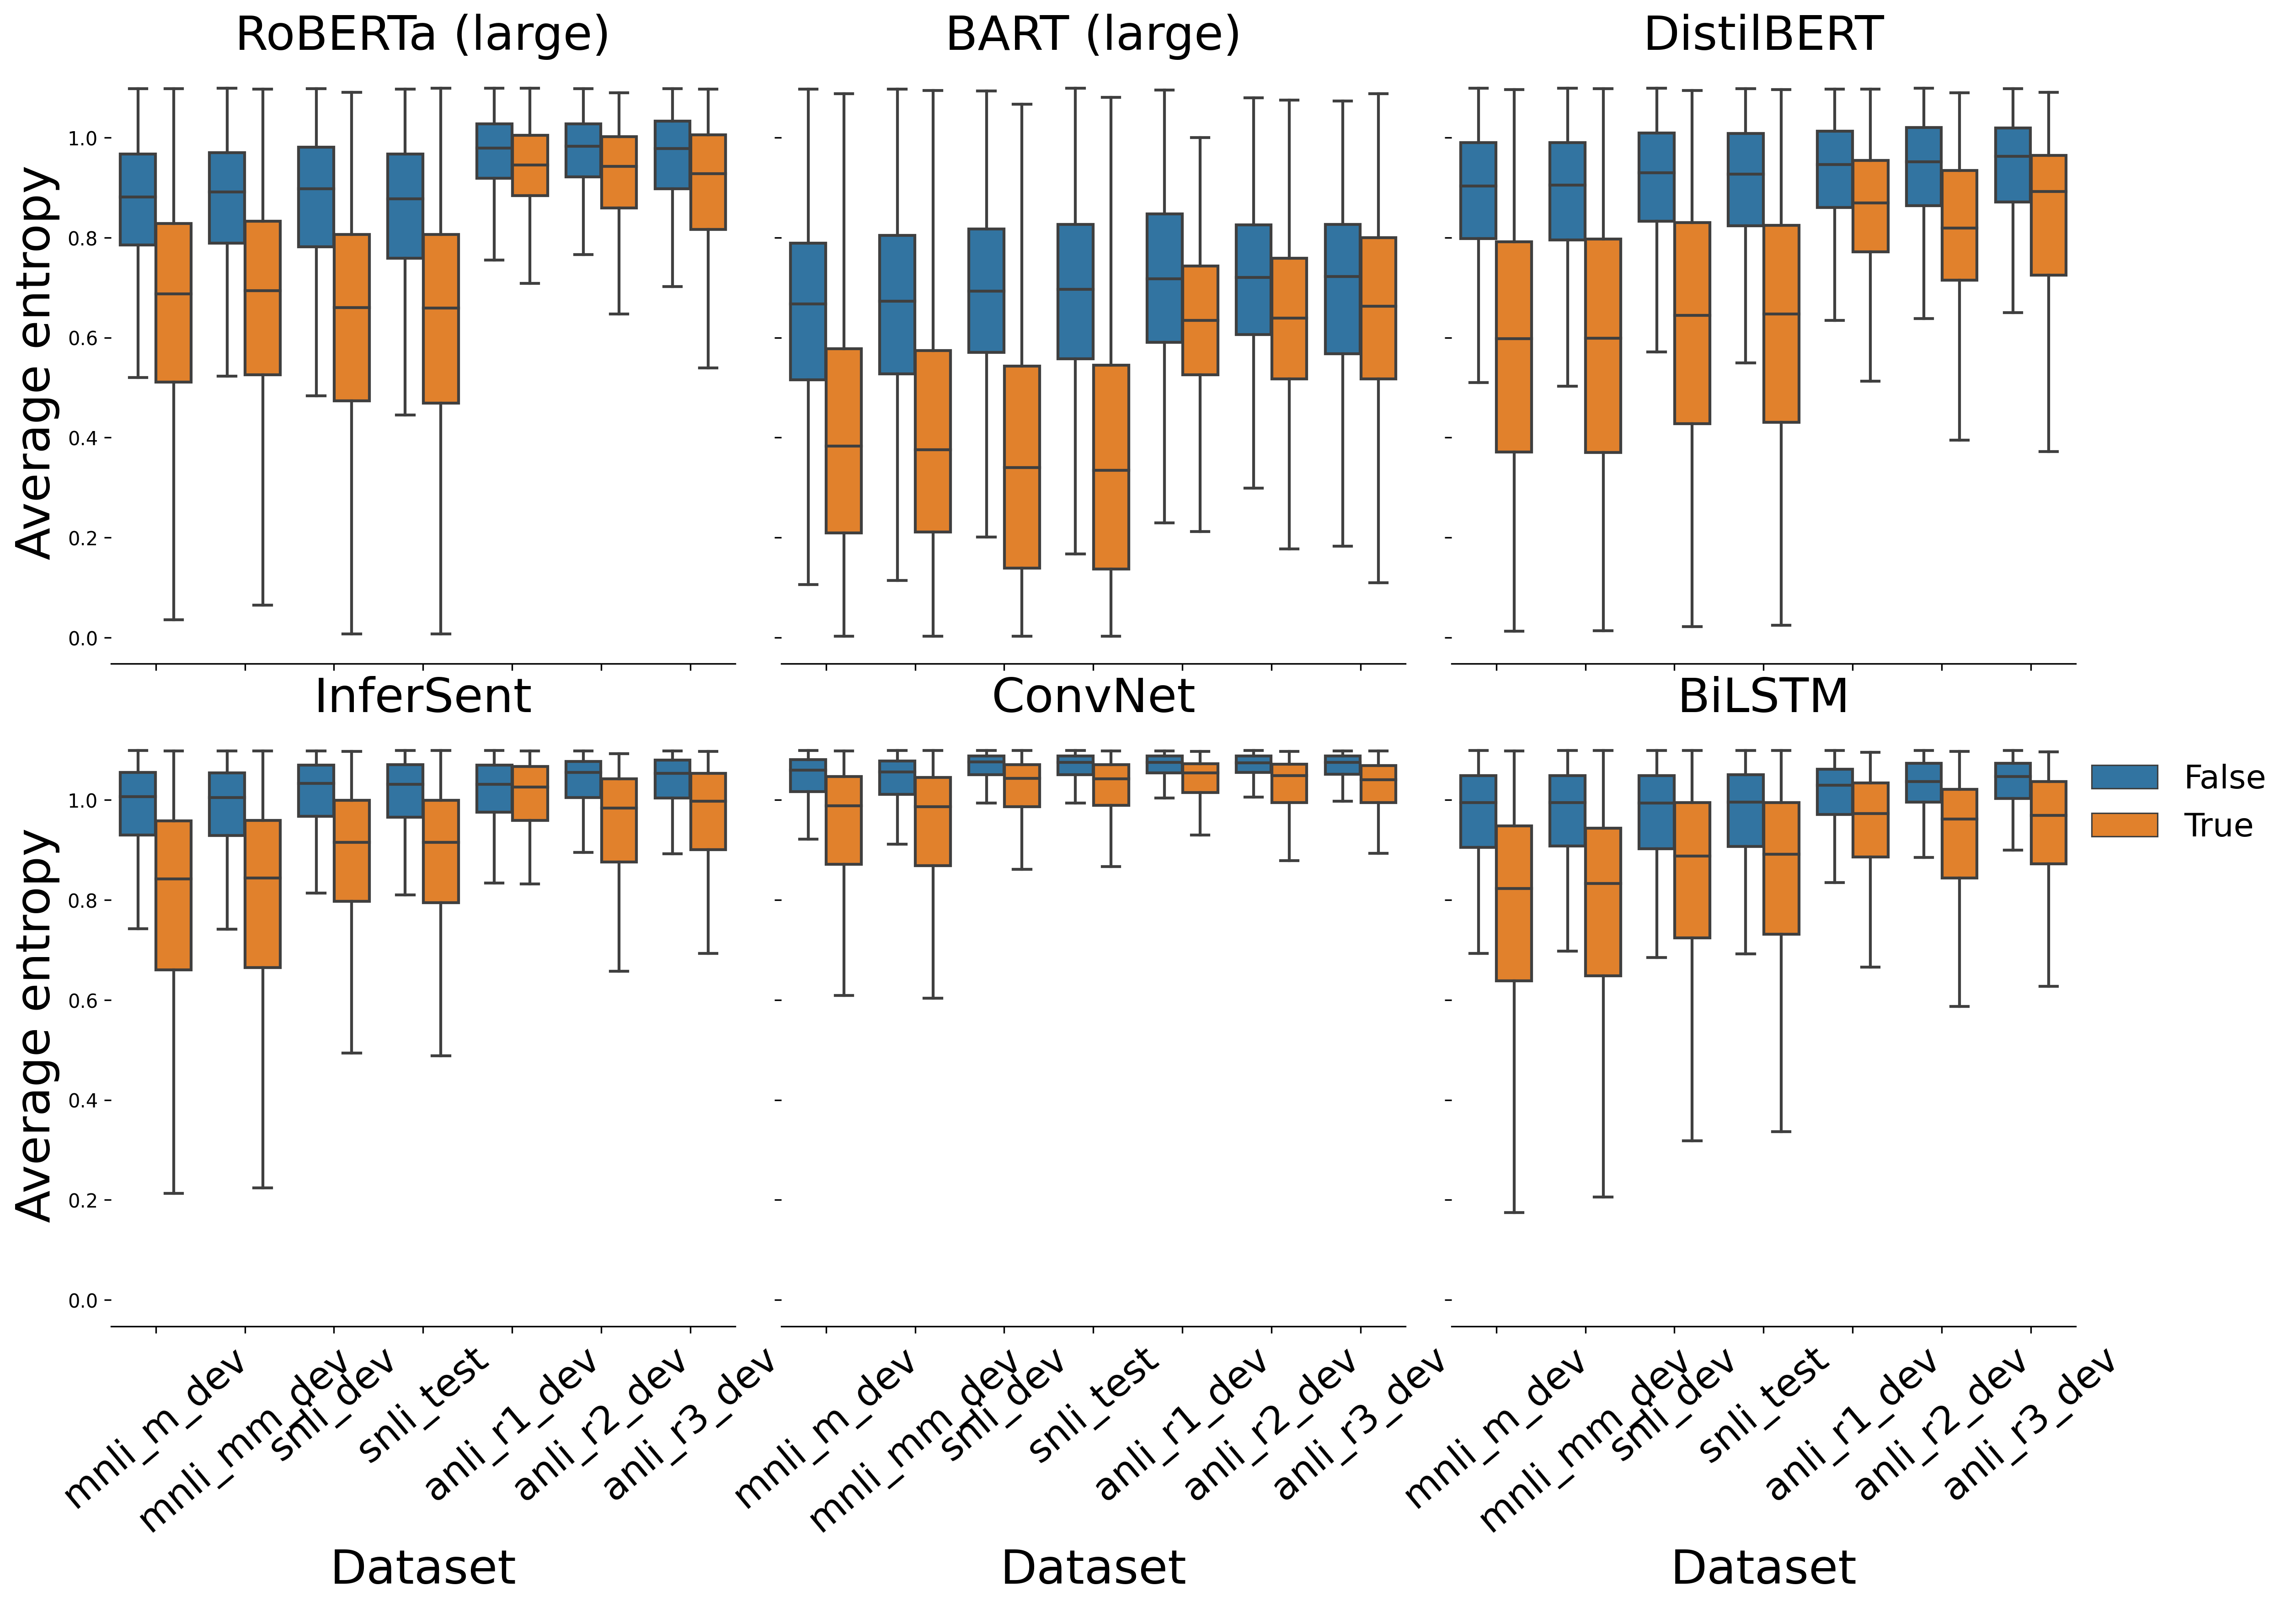
\includegraphics[width=0.48\textwidth]{images/unli_entropy_plot.png}
\end{center}
\caption{Model confidences on unnatural input}
\label{fig:all_entropy}
\end{wrapfigure}


The phenomenon we observe would be of less concern if the correct label prediction was just an outcome of chance, which could occur when the entropy of the log probabilities of the model output is high (suggesting uniform probabilities on entailment, neutral and contradiction labels). We first investigate the model probabilities for the Transformer-based models on the permutations that lead to the correct answer in \autoref{fig:all_entropy}. We find overwhelming evidence that model confidences on in-distribution datasets (MNLI, SNLI) are highly skewed, resulting in low entropy, and it varies among different model types. BART proves to be the most skewed Transformer-based model. This skewness is not a property of model capacity, as we observe DistilBERT log probabilities to have similar skewness as RoBERTa (large) model, while exhibiting lower model accuracy, maximum accuracy, and random accuracy.

\xit{How does humans perform on permuted examples?}

We expect humans to struggle with unnatural data, given our intuitions and the sentence superiority findings \cite{mollica-2020-composition}. To test this, we presented two experts in NLI (one a linguist) with permuted sentence pairs to label.\footnote{Concurrent work \cite{gupta-etal-2021-bert} found that untrained crowdworkers accept NLI examples that have been subjected to different kinds of perturbations at roughly most frequent class levels---i.e., only 35\% of the time.} Concretely, we draw equal number of examples from MNLI Matched dev set (100 examples where RoBERTa predicts the gold label, $D^c$ and 100 examples where it fails to do so, $D^f$), and then permute these examples using $\mathcal{F}$. The experts were given no additional information (recall that it is common knowledge that NLI is a roughly balanced 3-way classification task). Unbeknownst to the experts, all permuted sentences in the sample were actually accepted by the RoBERTa (large) model (trained on MNLI dataset). We observe that the experts performed much worse than RoBERTa (58.1\% and 37.8\%), although their accuracy was a bit higher than random. We also find that for both experts, accuracy on permutations from $D^c$ was higher than on $D^f$, which verifies findings that showed high word overlap can give hints about the ground truth label \citep{dasgupta-etal-2018-evaluating, poliak-etal-2018-hypothesis, gururangan-etal-2018-annotation, naik-etal-2019-exploring}.


\subsubsection{Discussion}

We show that state-of-the-art models do not rely on sentence structure the way we think they should: NLI models (Transformer-based models, RNNs, and ConvNets) are largely insensitive to permutations of word order that corrupt the original syntax. This raises questions about the extent to which such systems understand ``syntax'', and highlights the unnatural language understanding processes they employ.
We also show that reordering words can cause models to flip classification labels. % future work could additionally explore the relationship between permutation and deletion.
We do find that models seem to have learned some syntactic information (we observed a correlation between preservation of abstract POS neighborhood information and rate of acceptance by models, please refer to the paper for more details) but these results do not discount the high rates of permutation acceptance, and require further verification. Coupled with the finding that humans cannot perform UNLI at all well, the high rate of permutation acceptance that we observe leads us to conclude that current models do not yet ``know syntax'' in the fully systematic and humanlike way we would like them to.


\subsection{Masked Language Modeling and the Distributional Hypothesis: \textit{Order word matters pre-training for little}}

\subsubsection{Motivation}

In our previous work, we uncovered the unsystematic language understanding mechanisms employed by large, pre-trained NLU models, as they accept permuted sentences in surprising quantity. This questions the claims recently proposed in the literature that these models ``rediscovers the classical NLP pipeline'', suggesting that BERT-based models have the necessary inductive bias to learn syntax representations from self-supervised pre-training. Thus, we investigate further on the fact that how much of language models (specifically, Masked Language Models (MLM)) success is attributed to its knowledge of semantic and syntactic abstractions of natural language \cite{sinha2021a}. To do so, we measure the effect of removing word order during pre-training, with the assumption that any sophisticated (English) NLP pipeline presumably dpeends on the important syntactic information conveyed by the order of words. Suprisingly, we find the most of MLM's high performance can in fact be explained by the ``distributional prior'' - its ability to model word co-occurrence statistics - rather than its ability to replicate the classical NLP pipeline.

\subsubsection{Experiments \& Results}

In our experiments, we pre-train MLMs~(RoBERTa, \cite{liu2019b}) on various corpora with permuted word order while preserving some degree of distributional information, and examine their downstream performance.
In our main experiments, we pre-train models on various permuted corpora , by randomly shuffling $n$-grams within the sentence (where $n \in \{1,2,3,4\}$).
We also experiment with training MLMs without positional embeddings, making them entirely order agnostic,
and with training on a corpus sampled from the source corpus's %uniform or
unigram distribution, removing both distributional and word order information
. We then evaluate these ``permuted'' models in a wide range of settings and compare with regularly-pre-trained models.

Concretely, we use the original 16GB BookWiki corpus (the Toronto Books Corpus, \cite{zhu2015aligning}, plus English Wikipedia) from \cite{liu2019b}. We denote the model trained on the original, un-modified BookWiki corpus as \OR{} (for ``natural''). We use two types of word order randomization methods: permuting words at the sentence level, and resampling words at the corpus level. We also account for n-grams such as bigram, trigram and four-gram - i.e. we construct permuted sentences by randomly keeping n-grams unchanged. We train RoBERTa models on four permutation variants of BookWiki corpus, \RI, \RII, \RIII, \RIV\ for each $n$-gram value $ \in {\{1,2,3,4\}}$. More details on the process, along with the pseudo code and sample quality, are provided in our paper \cite{sinha2021a}. To further measure the effect of the distributional information, we construct baselines devoid of any distributional signal. Specifically, we train RoBERTa on a variants of BookWiki Corpus, \RC\, where all unigrams are sampled from the corpus according to their frequencies, removing the co-occurrence information (i.e destroying all sentence and paragraph information). We also inspect the usefulness of word order by training a RoBERTa model without positional embedding (\NP\ ) and inspect the strength of inductive bias only by using a randomly initialized RoBERTa model (\RT\ ).

\blankline

\xit{How does word order shuffled pre-trained models behave in downstream tasks?}

In order to measure the effect of word order shuffled pre-training, we compare the models in the GLUE and PAWS downstream tasks. The GLUE \cite{wang2018glue} benchmark is a collection of 9 datasets for evaluating natural language understanding systems, of which we use Corpus of Linguistic Acceptability \cite[CoLA,][]{cola_warstadt2019neural}, Stanford Sentiment Treebank \cite[SST,][]{sst2_socher2013recursive}, Microsoft Research Paragraph Corpus \cite[MRPC,][]{mrpc_dolan2005automatically}, Quora Question Pairs (QQP)\footnote{\href{http://data.quora.com/First-Quora-Dataset-Release-Question-Pairs}{http://data.quora.com/First-Quora-Dataset-Release-Question-Pairs}}, Multi-Genre NLI \cite[MNLI,][]{williams-etal-2018-broad}, Question NLI \cite[QNLI,][]{qnli_rajpurkar2016squad, qnli_2_demszky2018transforming}, Recognizing Textual Entailment \cite[RTE,][]{rte1_dagan2005pascal, rte2_haim2006second, rte3_giampiccolo2007third, rte5_bentivogli2009fifth}. The PAWS task \cite{zhang2019paws} consists of predicting whether a given pair of sentences are paraphrases. This dataset contains both paraphrase and non-paraphrase pairs with high lexical overlap, which are generated by controlled word swapping and back translation. Since even a small word swap and perturbation can drastically modify the meaning of the sentence, we hypothesize the randomized pre-trained models will struggle to attain a high performance on PAWS. We fine-tune all models according to RoBERTa best practices.

\begin{wrapfigure}{r}{0.5\textwidth}
\begin{center}
  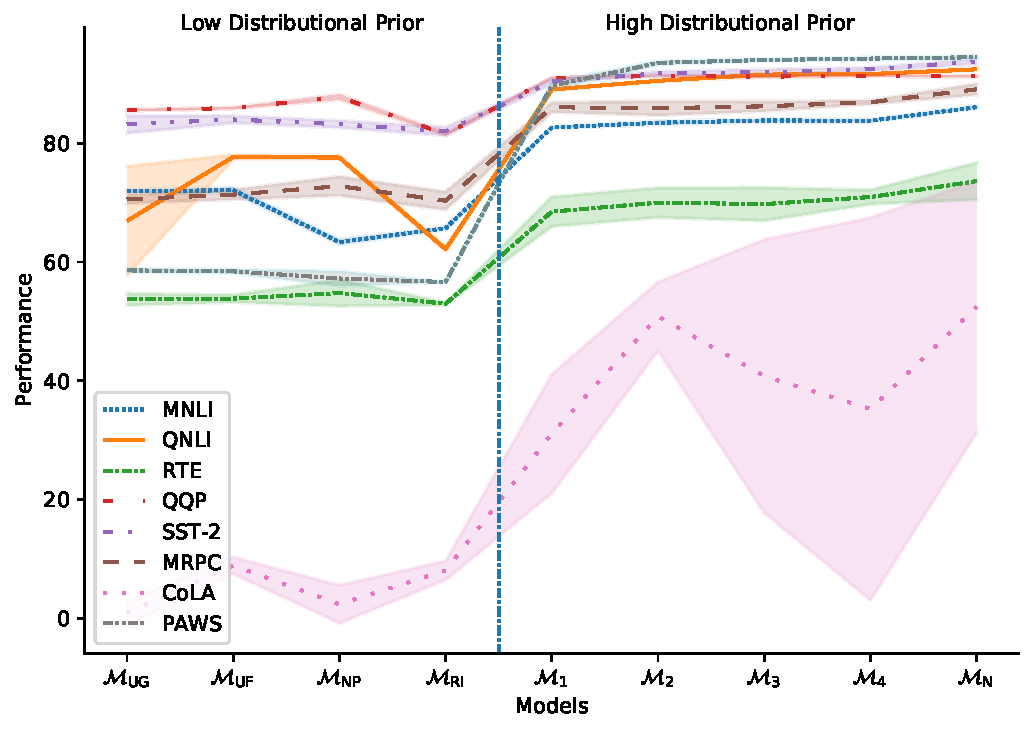
\includegraphics[width=0.48\textwidth]{images/masked_result.pdf}
\end{center}
\caption{Fine-tuning results on various word shuffled pre-trained models.}
\label{fig:masked_results}
\end{wrapfigure}


\textit{We observe that fine-tuning on word order shuffled pre-trained models perform remarkably close to the natural word order pre-trained model in case of all tasks.} \RI, the model pre-trained on completely shuffled sentences, is on average only $3.3$ points lower than \OR\ on the accuracy-based tasks,
and within $0.3$ points of \OR\ on QQP.
Even on PAWS, which was designed to require knowledge of word order, \RI\ is within $5$ points of \OR.
Randomizing $n$-grams instead of words during pre-training results in a (mostly) smooth increase on these tasks: \RIV, the model pre-trained on shuffled $4$-grams, trails \OR\ by only $1.3$ points on average, and even comes within $0.2$ points of \OR\ on PAWS. We observe a somewhat different pattern on CoLA, where \RII\ does almost as well as \OR\ and outperforms \RIII\ and \RIV, though we also observe very high variance across random seeds for this task.
Crucially, we observe that \RI\ outperforms \NP\ by a large margin. This shows that positional embeddings are critical for learning, even when the word orders themselves are not natural.
Overall, these results confirm our hypothesis that RoBERTa's strong performance on downstream tasks can be explained for a large part by the distributional prior.


\xit{Where does the models learn word order, in pre-training or in fine-tuning?}

There are two possible explanations for the above results: either the tasks do not need word order information to be solved, or any necessary word order information can be acquired during fine-tuning.
To examine this question, we permute the word order during fine-tuning as well. Concretely, for each task, we construct a unigram order-randomized version of each example in the fine-tuning training set using $\mathcal{F}_1$. We then fine-tune our pre-trained models on this shuffled data and evaluate task performance.

We observe for some taks (QQP, QNLI, MNLI, SST-2 and MRPC) the accuracy is still significantly high when fine-tuned on shuffled data, suggesting that purely lexical information is quite useful on its own. On the other hand, for the rest of the datasets (CoLA, PAWS, RTE) we observe noticable drops in accuracy when fine-tuned on shuffled data and tested on normal word order data, both for \OR\ and for shuffled models \RI\ through \RIV.
This suggests both that word order information is useful for these tasks, and that shuffled models must be learning to use word order information during fine-tuning. Having word order during fine-tuning is especially important for achieving high accuracy on CoLA, RTE (cf. \cite{pham2020}), as well as PAWS,
suggesting that these tasks are the most word order reliant.


\xit{How does syntactical probes behave when evaluated on word order shuffled pre-trained models?}

Since majority of the works investigating syntax representation use probes, we also employ similar mechanisms to test whether these probes are capable to differentiate the pre-trained models trained on shuffled word order from natural word order. In case of parametric probes (i.e probes having a learnable component), we use the Pareto optimality probing framework \cite{pimentel2020b} to investigate syntax using Dependency Parsing as an auxilliary task. By investigating the Dependency parsing task on two datasets (Penn Tree Bank and Universal Dependencies EWT), we observe that the results \textit{follow a similar trend as our downstream fine-tuning results} (Table \ref{tab:pareto_dependency}). Surprisingly, \RC\ probing scores seem to be somewhat better than \RI\ (though with large overlap in their standard deviations), even though \RC\ cannot learn information related to either word order or co-occurrence patterns.

\begin{wraptable}{r}{0.5\textwidth}
\resizebox{0.5\textwidth}{!}{%
\begin{tabular}{l|rl|rl}
\toprule
Model & \multicolumn{2}{c|}{UD EWT} & \multicolumn{2}{c}{PTB} \\ \hline
 & MLP & Linear & MLP & Linear \\ \cline{2-5} 
\OR & 80.41 +/- 0.85 & 66.26 +/- 1.59 & 86.99 +/- 1.49 & 66.47 +/- 2.77 \\\midrule
\RIV & 78.04 +/- 2.06 & 65.61 +/- 1.99 & 85.62 +/- 1.09 & 66.49 +/- 2.02 \\
\RIII & 77.80 +/- 3.09 & 64.89 +/- 2.63 & 85.89 +/- 1.01 & 66.11 +/- 1.68 \\
\RII & 78.22 +/- 0.88 & 64.96 +/- 2.32 & 84.72 +/- 0.55 & 64.69 +/- 2.50 \\
\RI & 69.26 +/- 6.00 & 56.24 +/- 5.05 & 79.43 +/- 0.96 & 57.20 +/- 2.76 \\\midrule
\RC & 74.15 +/- 0.93 & 65.69 +/- 7.35 & 80.07 +/- 0.79 & 57.28 +/- 1.42 \\
\bottomrule
\end{tabular}%
}
\caption{Unlabeled Attachment Score (UAS) (mean and std) on the dependency parsing task (DEP) on two datasets, UD EWT and PTB, using the Pareto Probing framework \cite{pimentel2020b}.}
\label{tab:pareto_dependency}
\end{wraptable}


We also find similar inconsistencies when analyzed with a suite of 10 probing tasks~\cite{conneau-etal-2018-cram} available in the SentEval toolkit~\cite{conneau-kiela-2018-senteval}. This suite contains a range of semantic, syntactic and surface level tasks. We observe that the \OR\ pre-trained model scores better than the unnatural word order models for \textit{only one out of five semantic tasks and in none of the lexical tasks}, unlike the claim of syntax understanding of BERT in the literature \cite{jawahar2019a}. However, \OR\ does score higher for two out of three syntactic tasks. Even for these two syntactic tasks, the gap among \RC\ and \OR\ is much higher than \RI\ and \OR. These results show that while natural word order is useful for at least some probing tasks, the distributional prior of randomized models alone is enough to achieve a reasonably high accuracy on syntax sensitive probing.


From our results so far, it is unclear whether parametric probing meaningfully distinguishes models trained with corrupted sentence order from those trained with normal orders. Thus, we also investigate non-parametric probes~\cite{linzen-etal-2016-assessing,marvin-linzen-2018-targeted,gulordava2018,goldberga,wolf2019}. Since these probes do not contain any learnable parameters, they are called ``non-parametric''. We observe for some datasets \cite{linzen-etal-2016-assessing,marvin-linzen-2018-targeted} the gap between the \OR\ and randomization models is relatively large.
While some randomization models (e.g., \RII, \RIII, and \RIV) performed quite similarly to \OR\ according to the parametric probes, they all are markedly worse than \OR\ according to the non-parametric ones. This suggests that non-parametric probes identify certain syntax-related modeling failures
that parametric ones do not.

\subsubsection{Discussion \& Conclusion}

The assumption that word order information is crucial for any classical NLP pipeline (especially for English) is deeply ingrained in our understanding of syntax itself \citep{chomsky1957syntactic}: without order, many linguistic constructs are undefined. % (e.g.\ dependency or constituency parses would no longer be syntactic trees, what would sentences be but mere lists of words).
Our fine-tuning results in \autoref{subsec:glue_results} and parametric probing results in \autoref{subsec:param_probing}, however, suggests that MLMs do not need to rely much on word order to achieve high accuracy, bringing into question previous claims that they learn a ``classical NLP pipeline''. These results should hopefully encourage the development of better, more challenging tasks that require sophisticated reasoning, and harder probes to narrow down what exact linguistic information is present in the representations learned by our models.





\section{Future Work \& Timeline}

Until now, most of the work in my doctoral studies have been focused on developing methods to detect the issue of systematicity plaguing neural NLU models. To complete my thesis, I thereby plan to work towards a couple of methods to improve robustness and systematicity of NLU models.

\subsection{Unsupervised syntax learning by mutually exclusive training using word order}

In our prior work on word order (Section \ref{sec:cont2}), we observed that NLU models are largely distributional - they understand the collection of words in a sentence but have limited understanding on the order of words. This poses a problem - representations of random permutations of the sentence having no grounded meaning will still be identified by the NLU models to contain syntactic and semantic information. Due to this distributional effect, we posit that syntax understanding of NLU models are still primitive, mostly restricted to higher order information. Thus, it is imperative to develop mechanisms to imbibe the required syntactical information within the sentence representation, such that it is systematic. One can use syntactic features such as dependency parses to imbibe information about syntax in the sentence representation using auxilliary supervison loss. In literature, such syntactical information has shown to be effective in downstream tasks, such as Relation Extraction (RE) \cite{fundel2007relex}, named entity recognition (NER) \cite{jie2019dependency} and semantic role labeling (SRL) \cite{strubell2018}. More recently, syntax trees are used during pre-training of Transformer based models to imbibe better syntactical information by early and late fusion \cite{sachan2021}. However, such direct supervision models to imbibe syntactical information is difficult as it requires access to preferably human-annotated syntax parses of sentences, which raises questions on the viability of such approaches for real world applications. Even so, limited studies have been performed to investigate systematicity issues of those models trained with supplementary syntactical signal.

Therefore, we propose an alternate, unsupervised mechanism to imbibe syntax information within the sentence representations by leveraging word order. Concretely, we use an auxilliary objective to the model to recognize correct and incorrect permutations of a given sentence alongside the task objective. Now, in the strictest sense there is only one correct ordering of a sentence which conveys the intended meaning. However, natural language (English) allows for a degree of flexibility in word order. Thus, we plan to leverage the idea of \textit{separable permutations} \cite{stanojevic2021}, where a subset of permutations can be treated as positive signal which can be reconstructed from the CCG parse of the given sentence. This auxilliary training loss could potentially inform the model to be systematic in understanding syntax, and thereby reduce the distributional, bag-of-words behavior of the encoder representations.

% Note: potential question from comittee: While this approach still requires a CCG parser, due to the nature of separable permutations this parser need not be perfect.

\subsection{Nonsensical data augmentation for better systematic generalization}

Systematic generalization is an issue which plagues many NLU tasks, in particular Natural Language Inference (NLI). Generalization to out-of-domain examples is poor \cite{nie2020}, and it has been shown that these models leverage the statistical artifacts in NLI datasets, such as SNLI and MNLI \cite{gururangan2018a}. One reason why models tend to overfit on the training data is the exposure bias to specific nouns/verbs/entities during training. When subjected to systematic stress test, the NLU models tend to be brittle as they fail to learn syntax of the training signal by fixating on the rare words and artifacts. Thus, we propose a dynamic data augmentation training scheme for NLU models where we repeat the training examples with word replacements from the same syntactic family. Overall, a sentence might lose its intended meaning (hence, ``nonsensical'') - however if the same operation is conducted on the premise, the entailment logic remains unchanged. Concretely, given a lexical item in a sentence, we randomly replace that item with another belonging to the same syntactic family, equally in both premise and hypothesis sentences. For empirical reasons we will restrict this replacement to specific family of lexicons (proper nouns, verbs) which typically form as rare elements in the dataset. We also plan to include a probabilistic model for this replacement which replaces lexicons based on their corpus probability to ensure uniformity in training. By systematically replacing the lexicons in a different context one can potentially increase the training data to reduce exposure bias problem. Similar methods have been devised for mitigating gender bias previously in the literature with varying success \cite{maudslay2020b}.

\subsection{Timeline}

\noindent \textbf{Unsupervised syntax learning by mutually exclusive training using word order} (1) Investigate CCG parsing to generate separable permutations on the fly, (2) Representational analysis on separable and non separable permutations, (3) Train auxillary loss with either direct supervision or partial gradient based methods such as Meta Learning, (4) Write paper for ACL 2022 or TACL 2022

\halfblankline

\noindent \textbf{Nonsensical data augmentation for better systematic generalization} (1) Investigate lexicon replacements by using syntactic parsers in a given dataset, (2) Analyze how the distribution of rare elements change in the training corpus by using this kind of replacement, (3) Test on out-of-domain data and NLI stress test sets, such as HANS \cite{mccoy2019}, (4) Write paper for EMNLP 2022.

\halfblankline

\noindent \textbf{Thesis preparation and submission} Expected defense date: Fall 2022

% Table if needed
% \begin{table}
% \centering
% \begin{tabular}{p{5cm}p{7cm}p{3cm}}
% Project & Task & Timeline\\
% \toprule
% Unsupervised syntax learning by mutually exclusive training using word order & \tabitem Investigate CCG parsing to generate separable permutations on the fly & \\
%  & \tabitem Representational analysis on separable and non separable permutations & \\
%  & \tabitem Train auxillary loss with either direct supervision or partial gradient based methods such as Meta Learning & \\
%  & \tabitem Write paper for ACL 2022 or TACL 2022 & \\
% Nonsensical data augmentation for better systematic generalization & \tabitem Investigate lexicon replacements by using syntactic parsers in a given dataset & \\
%  & \tabitem Analyze how the distribution of rare elements change in the training corpus by using this kind of replacement & \\
%  & \tabitem Test on out-of-domain data and NLI stress tests, such as HANS & \\
%  & \tabitem Write paper for EMNLP 2022 & \\
% \end{tabular}
% \end{table}


\bibliography{main}

\end{document}
